% CraftBot agent team organigram
% Build:  pdflatex craftbot_agent_team_organigram.tex
%         pdftoppm -png -r 200 craftbot_agent_team_organigram.pdf craftbot_agent_team_organigram
% Note: a \\ line break must sit at the top level of a node's text. Nesting one
% inside braces breaks TikZ's align=center, so each role line is its own group
% and the breaks stay outside them.
% Pure black and white, no dashes, one outline weight for every box.
% Spawn edges leave a box on the left, report edges return on the right, and
% every report edge carries the hand-off it delivers (README, agent team table).
\documentclass[border=12pt]{standalone}
\usepackage[T1]{fontenc}
\usepackage{mathptmx}
\usepackage{tikz}
\usetikzlibrary{positioning,arrows.meta,calc}

\newcommand{\agentname}[1]{{\bfseries\large #1}}
\newcommand{\role}[1]{{\itshape\small #1}}

\begin{document}
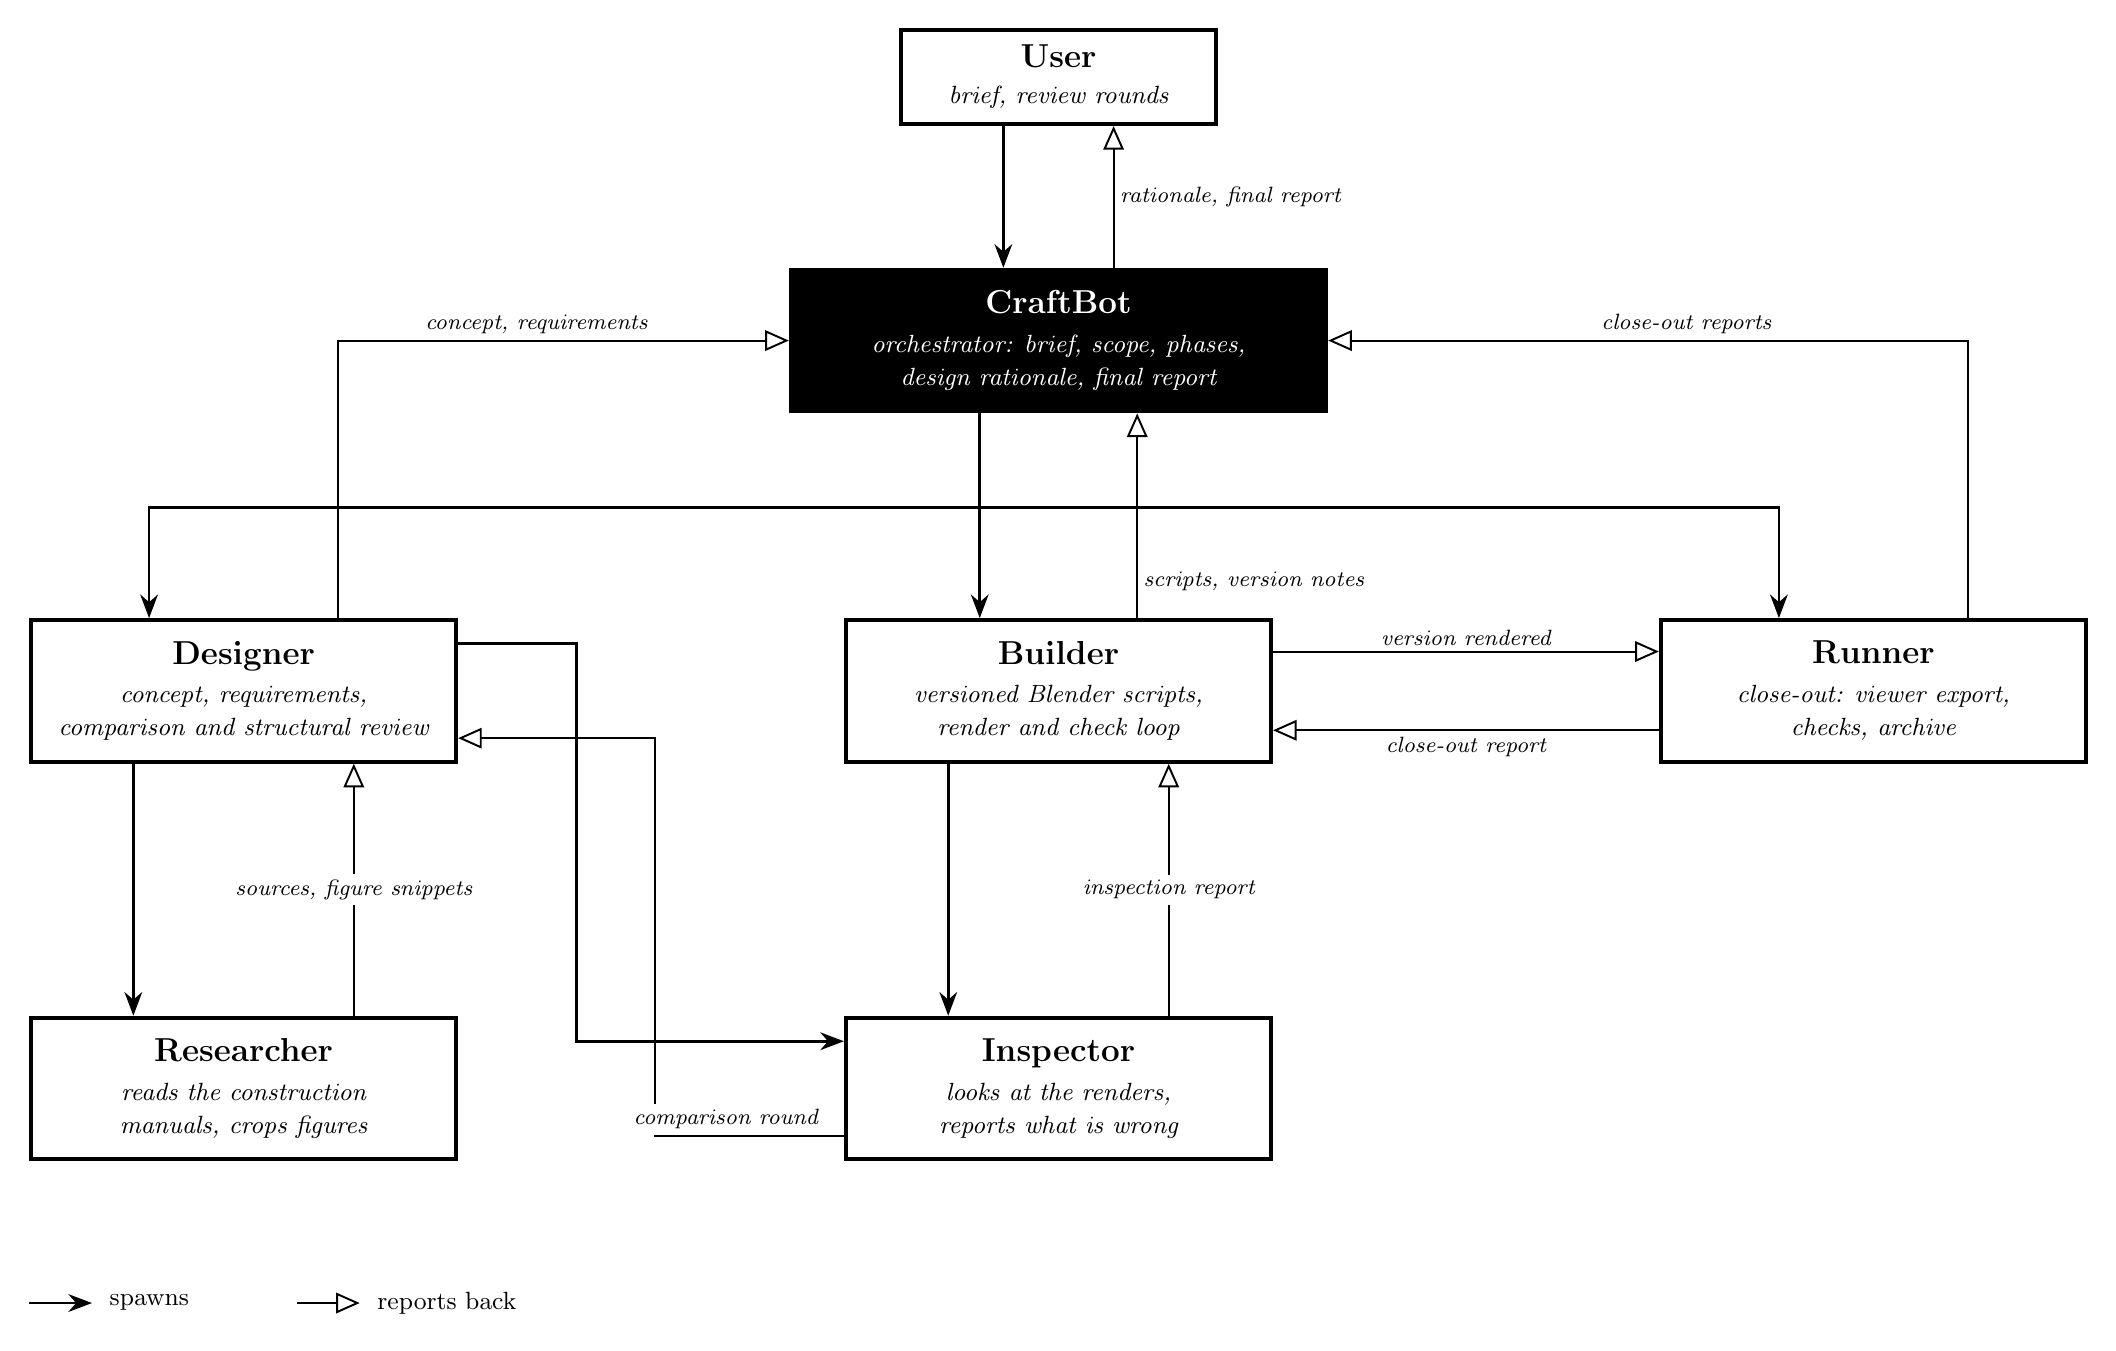
\begin{tikzpicture}[
  font=\rmfamily,
  agent/.style={rectangle, draw=black, line width=1.4pt, fill=white,
    minimum width=54mm, minimum height=18mm, align=center, inner sep=4pt, text=black},
  lead/.style={agent, fill=black, text=white, minimum width=68mm},
  human/.style={agent, minimum width=40mm, minimum height=12mm},
  spawn/.style={-{Stealth[length=3mm]}, draw=black, line width=1pt},
  report/.style={-{Triangle[length=3mm, width=2.6mm, open]}, draw=black, line width=0.7pt},
  edgelabel/.style={font=\rmfamily\itshape\footnotesize, text=black, inner sep=2pt,
    fill=white},
]

% ---- nodes ----
\node[human] (user) {\agentname{User}\\[1pt]\role{brief, review rounds}};

\node[lead, below=18mm of user] (craftbot)
  {\agentname{CraftBot}\\[2pt]\role{orchestrator: brief, scope, phases,}\\\role{design rationale, final report}};

\node[agent, below left=26mm and 42mm of craftbot] (designer)
  {\agentname{Designer}\\[2pt]\role{concept, requirements,}\\\role{comparison and structural review}};

\node[agent, below=26mm of craftbot] (builder)
  {\agentname{Builder}\\[2pt]\role{versioned Blender scripts,}\\\role{render and check loop}};

\node[agent, below right=26mm and 42mm of craftbot] (runner)
  {\agentname{Runner}\\[2pt]\role{close-out: viewer export,}\\\role{checks, archive}};

\node[agent, below=32mm of designer] (researcher)
  {\agentname{Researcher}\\[2pt]\role{reads the construction}\\\role{manuals, crops figures}};

\node[agent, below=32mm of builder] (inspector)
  {\agentname{Inspector}\\[2pt]\role{looks at the renders,}\\\role{reports what is wrong}};

% ---- spawn edges (left of centre) ----
\draw[spawn] ($(user.south)+(-7mm,0)$) -- ($(craftbot.north)+(-7mm,0)$);

\draw[spawn] ($(craftbot.south)+(-10mm,0)$) -- ($(builder.north)+(-10mm,0)$);
\draw[spawn] ($(craftbot.south)+(-10mm,0)$) -- ++(0,-12mm) -| ($(designer.north)+(-12mm,0)$);
\draw[spawn] ($(craftbot.south)+(-10mm,0)$) -- ++(0,-12mm) -| ($(runner.north)+(-12mm,0)$);

\draw[spawn] ($(designer.south)+(-14mm,0)$) -- ($(researcher.north)+(-14mm,0)$);
\draw[spawn] ($(builder.south)+(-14mm,0)$) -- ($(inspector.north)+(-14mm,0)$);
\draw[spawn] ($(designer.east)+(0,6mm)$) -| ($(inspector.west)+(-34mm,6mm)$)
             -- ($(inspector.west)+(0,6mm)$);

% ---- report edges (right of centre), each labelled with what it hands over ----
\draw[report] ($(craftbot.north)+(7mm,0)$) -- ($(user.south)+(7mm,0)$)
  node[edgelabel, midway, right] {rationale, final report};

\draw[report] ($(builder.north)+(10mm,0)$) -- ($(craftbot.south)+(10mm,0)$)
  node[edgelabel, pos=0.18, right] {scripts, version notes};

\draw[report] ($(designer.north)+(12mm,0)$) |- (craftbot.west)
  node[edgelabel, pos=0.72, above] {concept, requirements};

\draw[report] ($(runner.north)+(12mm,0)$) |- (craftbot.east)
  node[edgelabel, pos=0.72, above] {close-out reports};

\draw[report] ($(researcher.north)+(14mm,0)$) -- ($(designer.south)+(14mm,0)$)
  node[edgelabel, midway] {sources, figure snippets};

\draw[report] ($(inspector.north)+(14mm,0)$) -- ($(builder.south)+(14mm,0)$)
  node[edgelabel, midway] {inspection report};

\draw[report] ($(inspector.west)+(0,-6mm)$) -- ($(inspector.west)+(-24mm,-6mm)$)
  node[edgelabel, midway, above, xshift=-3mm] {comparison round}
  |- ($(designer.east)+(0,-6mm)$);

\draw[report] ($(builder.east)+(0,5mm)$) -- ($(runner.west)+(0,5mm)$)
  node[edgelabel, midway, above] {version rendered};

\draw[report] ($(runner.west)+(0,-5mm)$) -- ($(builder.east)+(0,-5mm)$)
  node[edgelabel, midway, below] {close-out report};

% ---- legend ----
\begin{scope}[shift={($(researcher.south west)+(0,-18mm)$)}]
  \draw[spawn] (0,0) -- (8mm,0);
  \node[anchor=west, font=\rmfamily\small, text=black] at (9mm,0) {spawns};
  \draw[report] (34mm,0) -- (42mm,0);
  \node[anchor=west, font=\rmfamily\small, text=black] at (43mm,0) {reports back};
\end{scope}

\end{tikzpicture}
\end{document}
